%!TEX root = ../../thesis.tex
\chapter{Reticulate Evolution in Pathogenic Bacteria}
\label{ch:pathogens}

\section{Introduction}
\label{pathogens:introduction}

Pathogenic bacteria can lead to severe infection and mortality and present an enormous burden on human populations and public health systems.
One of the achievements of twentieth century medicine was the development of a wide range of antibiotic drugs to control and contain the spread of pathogenic bacteria, leading to vastly increased life expectancies and global economic development.
However, rapidly rising levels of multidrug antibiotic resistance in several common pathogens, including \emph{Escherichia coli}, \emph{Klebsiella pneumoniae}, \emph{Staphylococcus aureus}, and \emph{Neisseria gonorrhoeae}, is recognized as a pressing global issue with near-term consequences \cite{Neu:1992gk,Thomas:2005hp,WHO:2014wa}.
The threat of a post-antibiotic 21st century is serious, and new methods to characterize and monitor the spread of resistance are urgently needed.

Antibiotic resistance can be acquired through point mutation or through horizontal transfer of resistance genes.
Horizontal exchange occurs when a donor bacteria transmits foreign DNA into a genetically distinct bacteria strain.
As discussed in Chapter~\ref{ch:background}, three mechanisms of horizontal transfer have been identified, depending on the route by which foreign DNA is acquired \cite{Ochman:2000dr}.
Foreign DNA can be acquired via uptake from an external environment (transformation), via viral-mediated processes (transduction), or via direct cell-to-cell contact between bacterial strains (conjugation).
Resistance genes can be transferred between strains of the same species, or can be acquired from different species in the same environment.
While the former is generally more common, an example of the latter is the phage-mediated acquisition of Shiga toxin in \emph{E. coli} in Germany in 2011 \cite{Rohde:2011ju}.
Elements of the bacterial genome that show evidence of foreign origin are called genomic islands, and are of particular concern when associated with phenotypic effects such as virulence or antibiotic resistance.

In this chapter we explore topics relating to horizontal gene transfer in bacteria and the emergence of antibiotic resistance in pathogenic strains.
We show that TDA can not only quantify gene transfer events, but also characterize the scale of gene transfer.
The scale of recombination can be measured from the distribution of birth times of the $H_1$ invariants in the barcode diagram.
It has been shown that recombination rates decrease with increasing sequence divergence \cite{Fraser:2007ep}.
We characterize the rate and scale of intraspecies recombination in several pathogenic bacteria of public health concern.
We select a set of pathogenic bacteria that are of public health interest based on a recently released World Health Organization (WHO) report on antimicrobial resistance \cite{WHO:2014wa}.
Using persistent homology, we characterize the rate and scale of recombination in the core genome using multilocus sequence data.
To extend our characterization to the whole genome, we use protein family annotations as a proxy for sequence composition.
This allows us to compute a similarity matrix between strains.
Comparing persistence diagrams gives us information about the relative scales of gene transfer at arbitrary loci.
The species selected for study and the sample sizes in each analysis are specified in Table~\ref{table:samplesizes}.
Next, we explore the spread of antibiotic resistance genes in \emph{S. aureus} using Mapper, an algorithm for partial clustering and visualization of high dimensional data \cite{Singh:2007ve}.
We identify two major populations of \emph{S. aureus}, and observe one cluster with strong enrichment for the antibiotic resistance gene \emph{mecA}.
Importantly, resistance appears to be increasingly spreading in the second population.
Finally, we consider the risk of lateral transfer of resistance genes from the human microbiome into an antibiotic sensitive strain, using $\beta$-Lactam resistance as an example.
In this environment, benign bacterial strains can harbor known resistance genes.
We use a network analysis to visualize the spread of antibiotic resistance gene $\emph{mecA}$ into nonnative phyla.
Each individual has a unique microbiome, and we speculate that microbiome typing of this sort may useful in developing personalized antibiotic therapies.
These results suggest an important role for topological data mining of -omics scale data in clinical applications and personalized medicine.

\begin{table}
\centering
\caption[List of pathogenic bacteria selected for study]{Pathogenic bacteria selected for study and sample sizes in each analysis.}
\begin{tabularx}{\textwidth}{Xcc}
\toprule
Species & \hspace{10mm}MLST profiles\hspace{10mm} & PATRIC profiles \\
\midrule
\emph{Campylobacter jejuni}      & 7216  & 91 \\
\emph{Escherichia coli}          & 616   & 1621 \\
\emph{Enterococcus faecalis}     & 532   & 301 \\
\emph{Haemphilus influenzae}     & 1354  & 22 \\
\emph{Helicobacter pylori}       & 2759  & 366 \\
\emph{Klebsiella pneumoniae}     & 1579  & 161 \\
\emph{Neisseria spp.}            & 10802 & 234 \\
\emph{Pseudomonas aeruginosa}    & 1757  & 181 \\
\emph{Staphylococcus aureus}     & 2650  & 461 \\
\emph{Salmonella enterica}       & 1716  & 638 \\
\emph{Streptococcus pneumoniae}  & 9626  & 293 \\
\emph{Streptococcus pyogenes}    & 627   & 48 \\
\bottomrule
\end{tabularx}
\label{table:samplesizes}
\end{table}

\section{Evolutionary Scales of Recombination in the Core Genome}
\label{pathogens:mlst}
%
Multilocus sequence typing (MLST) data was used to examine scales of recombination in the core bacterial genome.
MLST is a method of rapidly assigning a sequence profile to a sample bacterial strain.
For each species, a predetermined set of loci in a small number of housekeeping genes are selected as representative of the core genome of the species.
At each loci, a set of sequence types are defined by using a similarity-based clustering.
As new strains are sequenced, they are annotated with a profile corresponding to the type at each locus.
If a sample has a previously unseen type at a given locus, it is appended to the list of types at that locus.
Large online databases have curated MLST data from labs around the world; significant pathogens can have several thousand typed strains (over 10,000 in the case of \emph{Neisseria spp.}).
Because different species will be typed at different loci, examining direct interspecies genetic exchange with this data is unfeasible, however MLST provides a large quantity of data with which to examine intraspecies exchange in the core genome.
Finally, because the selected loci are primarily housekeeping genes, this type of recombination analysis will tell you only about genetic exchange in the core genome.
Mobile genetic elements may have a separate rates of exchange.

We investigate genetic exchange in the twelve pathogens using MLST data from PubMLST \cite{Jolley:2010gf}.
For each strain, a pseudogenome can be constructed by concatenating the typed sequence at each locus.
Using a Hamming metric, we construct a pairwise distance matrix between strains and compute persistent homology on the resulting metric space.
Because of the large number of sample strains, we employ a Lazy Witness complex with 250 landmark points and $\nu=0$ \cite{deSilva:2004tg}.
The computation is performed using javaplex \cite{Tausz:2011}.
An example of our output is shown in Figure~\ref{fig:pathogen_barcodes}, where we plot the $H_1$ barcode diagrams for \emph{K. pneumoniae} and \emph{S. enterica}.
The two species have distinct recombination profiles, characterized by the range of recombinations: \emph{K. pneumoniae} recombines at only an early short-lived scale, while \emph{S. enterica} recombines both at the short-lived scale and a longer-lived scale.
These multiple scales are reflective of population structure at the subspecies level: in \emph{S. enterica}, there are seven defined subspecies, and experimental studies have shown high levels of reticulation both within and between subspecies groups \cite{Brown:2003id}.
We repeat this analysis for each species, and plot the results as a persistence diagram in Figure~\ref{fig:pathogen_persistence_diagram}.
Among the bulk of pathogens there appears to be three major scales of recombination, a short-lived scale at intermediate distances, a longer-lived scale at intermediate distances, and a short-lived scale at longer distances.
We recover a pronounced pattern of reticulation at very short distances unique to \emph{H. Pylori}, which is consistent with earlier measurements of an unusually small size of DNA imports, reported in \cite{Falush:2001cd}.

\begin{figure}
    \centering
    \subbottom[\emph{Klebsiella pneumoniae}]{
        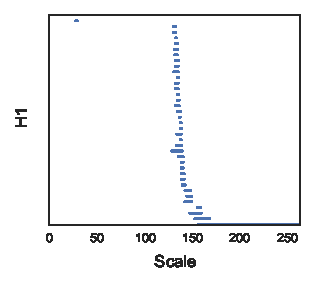
\includegraphics[width=.4\textwidth]{./fig/pathogens/kpneumoniae_barcode.pdf}}
    \subbottom[\emph{Salmonella enterica}]{
        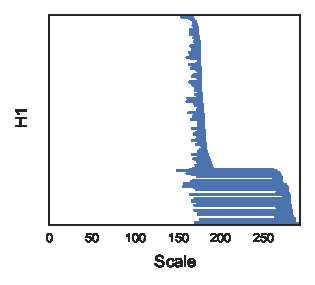
\includegraphics[width=.4\textwidth]{./fig/pathogens/senterica_barcode.pdf}}
    \caption[Core genome exchange in \emph{K. pneumoniae} and \emph{S. enterica}]{Barcode diagrams reflect different scales of core genomic exchange in \emph{K. pneumoniae} and \emph{S. enterica}. Differing scales can be attributed to different degrees of population substructure in the two species.}
    \label{fig:pathogen_barcodes}
\end{figure}

\begin{figure}
\centering
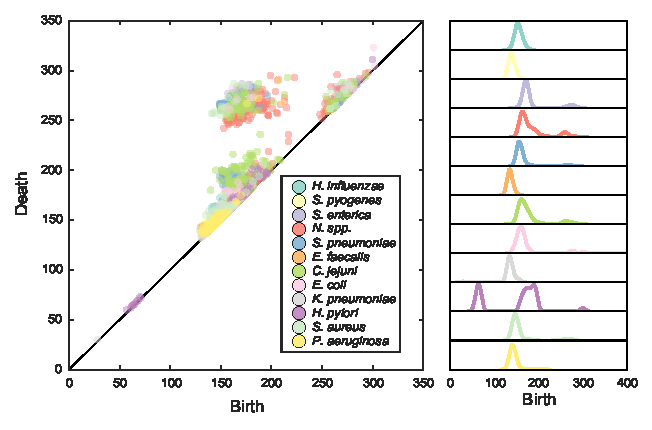
\includegraphics[width=\textwidth]{./fig/pathogens/pathogen_persistence_diagram.pdf}
\caption[$H_1$ persistence diagram for twelve pathogenic strains using MLST profile data]{The $H_1$ persistence diagram for the twelve pathogenic strains selected for this study using MLST profile data. There are three broad scales of recombination. To the right is the birth time distribution for each strain. \emph{H. pylori} has an earlier scale of recombination not present in the other species, corresponding to the atypically small size of DNA imports in the species \cite{Falush:2001cd}.}
\label{fig:pathogen_persistence_diagram}
\end{figure}

We define a relative rate of recombination by counting the total number of $H_1$ loops across the filtration and dividing by the number of samples for that species.
The results are shown in Figure~\ref{fig:pathogen_barchart}, where we observe that different species can have vastly different reticulation profiles.
For example, \emph{S. enterica} and \emph{E. coli} have the highest reticulation rates, consistent with earlier results which have shown a high proportion of defects in the \emph{mutS} mismatch-repair gene leading to relaxed genetic barriers to recombination \cite{Rayssiguier:1989gb,LeClerc:1996hx}.
The low measured reticulation rate in \emph{H. pylori} is a surprising outlier, as previous studies have shown that it lacks the mismatch repair pathways common in other bacteria, leading to higher than expected recombination rates \cite{Dorer:2011hx}.
\emph{H. pylori} has been reported to have very little clonal structure relative to other strains, which is reflected in the star-like phylogeny that has been proposed for the species \cite{Kalia:2004jx}
However, restriction-modification systems limiting uptake of foreign DNA have also been reported \cite{Dwivedi:2013bt}, suggesting that the \emph{H. pylori} core genome is relatively resistant to reticulation at wider genomic scales.
It is therefore plausible that the lower signal from persistent homology is due to systematic reduced sampling of particular lineages, suggesting that accounting for larger-scale population structure is important when making estimates of reticulation rates.

\begin{figure}
\centering
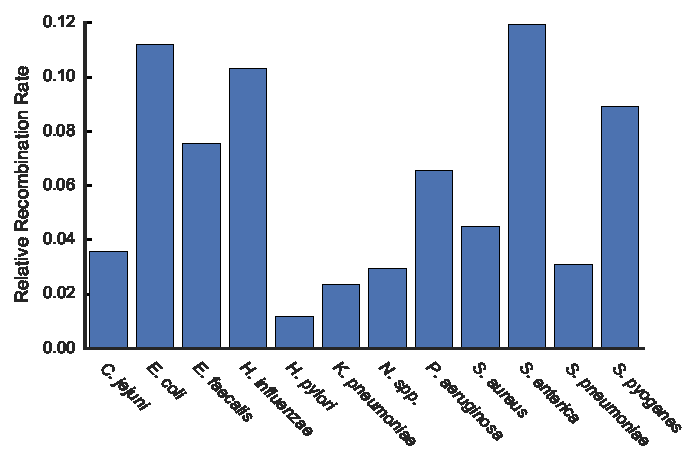
\includegraphics[width=\textwidth]{./fig/pathogens/pathogen_barchart.pdf}
\caption[Core genome reticulation patterns in pathogenic bacteria from MLST profiles]{Relative recombination rates computed by persistent homology from MLST profile data.}
\label{fig:pathogen_barchart}
\end{figure}

\section{Protein Families as a Proxy for Genome Wide Reticulation}
\label{pathogens:patric_analysis}

Protein family annotations cluster proteins into sets of isofunctional homologs, i.e., clusters of proteins with both similar sequence composition and similar function.
A particular strain is represented as a binary vector indicating the presence or absence of a given protein family.
Correlations between strains can reveal genome-wide patterns of genetic exchange, unlike the MLST data which can only provide evidence of exchange in the core genome.
We use the FigFam protein annotations in the Pathosystems Resource Institute Center (PATRIC) database because of the breadth of pathogenic strain coverage and depth of genomic annotations \cite{Wattam:2013jy}.
The FigFam annotation scheme consists of over 100,000 protein families curated from over 950,000 unique proteins \cite{Meyer:2009iq}.

For each strain we compute a transformation into FigFam space.
We transform into this space because the frequency of genome rearrangements and differences in mobile genetic elements makes whole genome alignments unreliable, even for strains within the same species.
As justification for performing this step, it has been shown experimentally that recombination rates decrease with increasing genetic distance \cite{Fraser:2007ep}.
After transforming, we construct a strain-strain correlation matrix and compute the persistent homology in this space.
In Figure~\ref{fig:figfam_persistence_diagram} we show the persistence diagram relating the structure and scale between different species.
We find that different species have a much more diverse topological structure in this space than in MLST space, and a wide variety of recombination scales.
The large scales of exchange in \emph{H. influenzae} suggest it can regularly acquire novel genetic material from distantly related strains.
% TODO: why? this is correlation across genome - very mosaic?

\begin{figure}
\centering
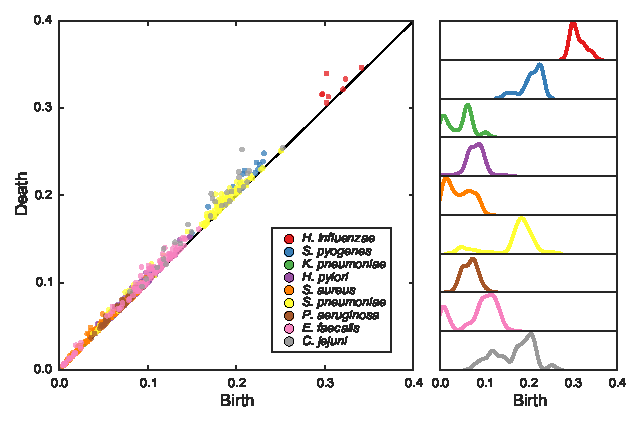
\includegraphics[width=\textwidth]{./fig/pathogens/figfam_persistent_diagram.pdf}
\caption[Genome-wide reticulation patterns in pathogenic bacteria from protein annotations]{Persistence diagram for a subset of pathogenic bacteria, computed using the FigFam annotations compiled from PATRIC. Compared to the MLST persistence diagrams, the Figfam diagrams have a more diverse scale of topological structure.}
\label{fig:figfam_persistence_diagram}
\end{figure}

\section{Antibiotic Resistance in \emph{Staphylococcus aureus}}
\label{sec:staph_aureus}
%
\emph{S. aureus} is a gram positive bacteria commonly found in the nostrils and upper respiratory tract.
Certain strains can cause severe infection in high-risk populations, particularly in the hospital setting.
The emergence of antibiotic resistant \emph{S. aureus} is therefore of significant clinical concern.
Methicillin resistant \emph{S. aureus} (MRSA) strains are resistant to $\beta$-lactam antibiotics including penicillin and cephalosporin.
Resistance is conferred by the gene \emph{mecA}, an element of the Staphylococcal cassette chromosome mec (\emph{SCCmec}).
\emph{mecA} codes for a dysfunctional penicillin-binding protein 2a (PBP2a), which inhibits $\beta$-lactam antibiotic binding, the primary mechanism of action \cite{Jensen:2009fu}.
Of substantial clinical importance are methods for characterizing the spread of MRSA within the \emph{S. aureus} population.

To address this question, we use the FigFam annotations in PATRIC, as described in the previous section.
PATRIC contains genomic annotations for 461 strains of \emph{S. aureus}, collectively spanning 3,578 protein families.
We perform a clustering analysis using the Mapper algorithm as implemented in Ayasdi Iris \cite{AyasdiIris:2015}.
Principal and second metric singular value decomposition are used as filter functions, with a 4x gain and an equalized resolution of 30.
This results in a graph structure with two large clusters, with a smaller bridge connecting the two, as shown in Figure~\ref{fig:saureus_figfam_network}.
The two clusters are consistent with previous phylogenetic studies using multilocus sequence data to identify two major population groups \cite{Cooper:2006dp}.

Of the 461 \emph{S. aureus} strains in PATRIC, 142 carry the \emph{mecA} gene.
When we color nodes in the network based on an enrichment for the presence of \emph{mecA}, we observe a much stronger enrichment in one of the two clusters.
This suggests that $\beta$-lactam resistance has already begun to dominate in that clade, likely due to selective pressures.
More strikingly, we observe that while \emph{mecA} enrichment is not as strong in the second cluster, there is a distinct path of enrichment emanating along the connecting bridge between the two clusters and into the less enriched cluster.
This suggests the hypothesis that antibiotic resistance has spread from the first cluster into the second cluster via strains intermediate to the two, and will likely continue to be selected for in the second cluster.

\begin{figure}[t]
\centering
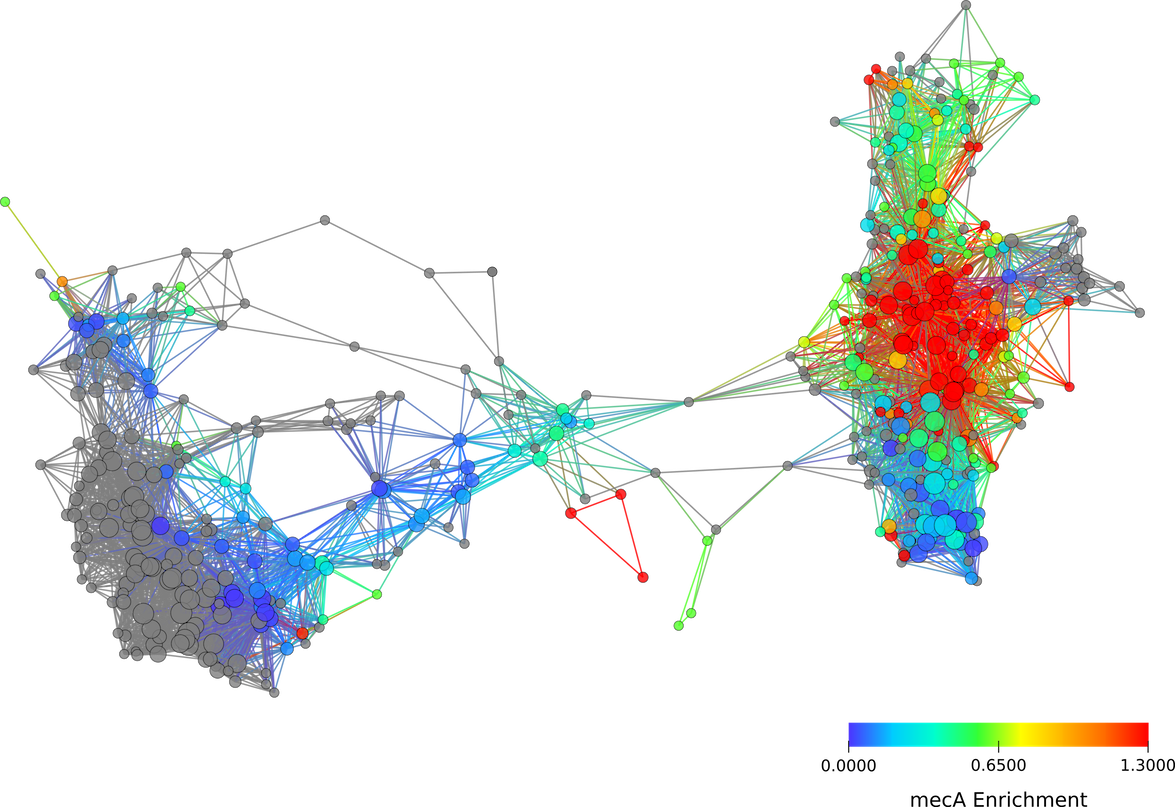
\includegraphics[width=\textwidth]{./fig/pathogens/saureus_figfam_network.png}
\caption[FigFam similarity network of \emph{S. aureus}]{The FigFam similarity network of \emph{S. aureus} constructed using Mapper as implemented in Ayasdi Iris \cite{AyasdiIris:2015}. We use a Hamming metric and Primary and Secondary Metric SVD filters (res: 30, gain 4x, equalize). Node color is based on strain enrichment for \emph{mecA}, the gene conferring $\beta$-Lactam resistance. Two distinct clades of \emph{S. aureus} are visible, one of which has already been compromised for resistance. Of important clinical significance is the growing enrichment for \emph{mecA} in the second clade.}
\label{fig:saureus_figfam_network}
\end{figure}

\section{Microbiome as a Reservoir of Antibiotic Resistance Genes}
\label{pathogens:microbiome}

While antibiotic resistance can be acquired through gene exchange between strains of the same species, it is also possible for gene exchange to occur between distantly related species.
It has been recognized that an individual's microbiome, the set of microorganisms that exist symbiotically within a human host, can act as a reservoir of antimicrobial resistance genes \cite{Sommer:2010uh,Penders:2013wt}.
It is of substantial clinical interest to characterize to what extent an individual's microbiome may pose a risk for a pathogenic bacteria acquiring a resistance gene through lateral transfer.

To address this question, we use data from the Human Microbiome Project (HMP), a major research initiative performing metagenomic characterization of hundreds of healthy human microbiome samples \cite{Consortium:2012bm}.
The HMP has defined a set of reference strains that have been observed in the human microbiome.
We collect FigFam annotations from PATRIC for the reference strain list in the gastrointestinal tract.
We focus on the gastrointestinal tract because it is an isolated environment and likely to undergo higher rates of exchange than other anatomic regions.
Of the 717 reference strains, 321 had FigFam annotations.
We computed a similarity matrix as in previous sections, using correlation as distance.
The resulting network is shown in Figure~\ref{fig:microbiome_network}, where strains are colored by phyla-level classifications.
While largely recapitulating phylogeny, the network depicts interesting correlations between phyla, such as the loop between Firmicutes, Bacteroides, and Proteobacteria.

Next, we searched for genomic annotations relating to $\beta$-lactam resistance.
10 strains in the reference set had matching annotations, and we highlight those strains in the network with green diamonds.
We observe resistance mostly concentrated in the Firmicutes, of which \emph{S. aureus} is a member, however there is a strain of Proteobacteria that has acquired the resistance gene.
Transfer of beta-lactam resistance into the Proteobacteria is clinically worrisome.
Pathogenic Proteobacteria include \emph{S. enterica}, \emph{V. cholerae}, and \emph{H. pylori}, and emergence of $\beta$-lactam resistance will severely impact antibiotic drug therapies.

The species composition of each individual's microbiome can differ substantially due to a wide variety of poorly understood factors \cite{Consortium:2012bm}.
In this case, an individuals personal microbiome network will differ from the network we show in Figure~\ref{fig:microbiome_network}, which was constructed from the set of \emph{all} strains that have been reported across studies of multiple individuals.
The relative risk for acquiring self-induced resistance will therefore vary from person to person and by the infectious strain acquired.
However, a network analysis of this type will give clues as to possible routes by which antibiotic resistance may be acquired.
In the clinical setting, this could assist in developing personalized antibiotic treatment regimens.
We propose a more thorough expansion of this work, examining the full range of antibiotic resistance genes in order to quantify microbiome risk factors for treatment failure.
We foresee an era of genomically informed infectious disease management in the clinical setting, based on an understanding of a patient's personal microbiome profile.

\begin{figure}[t]
\centering
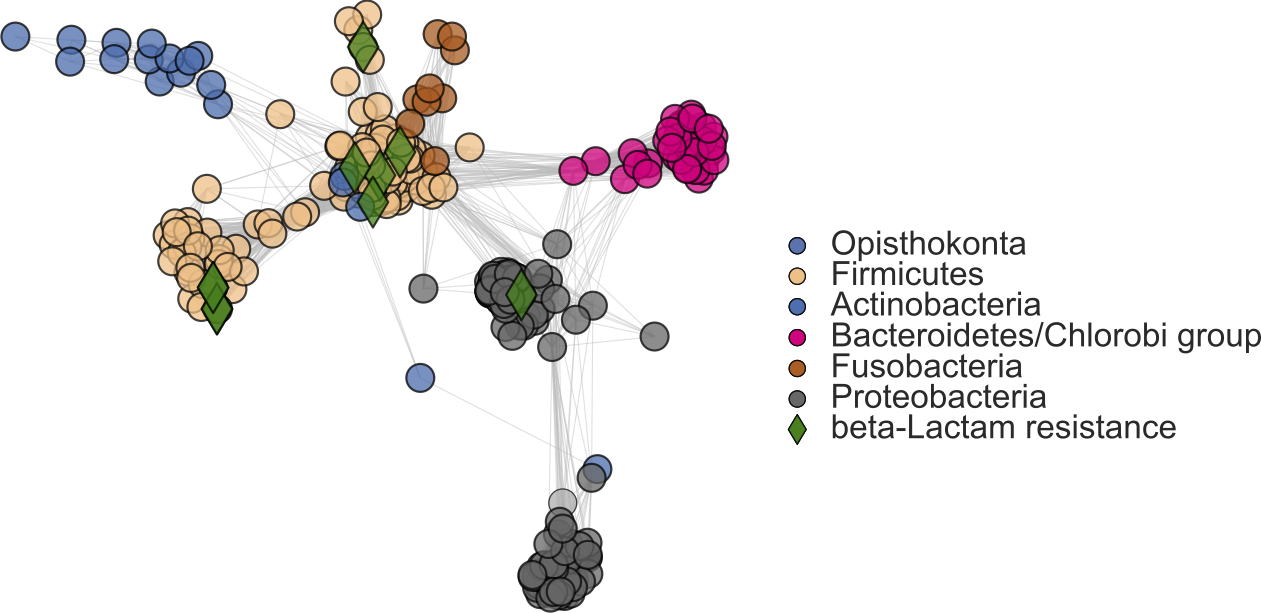
\includegraphics[width=\textwidth]{./fig/pathogens/microbiome_network.pdf}
\caption[FigFam similarity network of the gastrointestinal tract]{The FigFam similarity network of gastrointestinal tract reference strains identified in the Human Microbiome Project. The green diamond identifies the strains carrying resistance to $\beta$-Lactam antibiotics.}
\label{fig:microbiome_network}
\end{figure}

\section{Conclusions}

In this chapter we have used some ideas from topological data analysis to bear on problems in pathogenic microbial genetics.
First, we used persistent homology to evaluate recombination rates in the core genome using MLST profile data.
We showed that different pathogens have different recombination rates.
We expanded this to gene transfer across the whole genome by using protein family annotations in the PATRIC database.
We found different scales of recombination in different pathogens.
Second, we explored the spread of MRSA in \emph{S. aureus} populations using topological methods.
We noted increasing resistance in a previously isolated population.
Finally, we studied the emergence of $\beta$-lactam resistance in the microbiome, and proposed methods by which personal risk could be assessed by microbiome typing.
These results point to a role for graph mining and topological data mining in health and personalized medicine.